\chapter{Design}

\section{Introduction}
This chapter provides a description of the design decisions for the research project being conducted.
This builds upon the state of the art technology which was previously discussed in chapter 2.
In this chapter the requirements for the project are also discussed in relation to the objectives and challenges which were listed in chapter 1.
The overall system architecture will be presented in the form of UML diagrams.

\section{Requirements}
Based on the objectives and challenges as listed in chapter 1, the requirements can be split into corpus requirements and implementation requirements.
The corpus requirements deal with the selection of the corpus and sampling of the when test are run across different sizes of the corpus.
The implementation requirement deal with the three algorithms chosen and the different libraries used to implement them in the project.

\subsection{Corpus Selection}
In the context of generating recommendations for a student an academic or educational corpus should be used.
The availability of a large and respected educational corpus poises a problem however.
It was decided that academic papers from arXiv would act as a proxy for educational resources.
This in itself could create a problem due to how academic papers are usually written.
The language of an academic paper is usually quite different to the language used in a textbook or a lecture.
The language used is generally an advanced discussion of a particular subject, which itself could have it's own vocabulary.
This is particularly relevant for the arXiv corpus which has a large number of papers related to mathematics and physics.

While arXiv may not be the perfect educational corpus it is an adequate proxy.
The arXiv corpus could also be comparable to the corpus used by Blei in his paper on LDA.
In the Blei experiment, LDA was applied to approximately 22,000 articles from the journal Nature.
In that experiment Blei created an LDA model with 50 topics and used it to identify topics with documents and to find documents of a similar topic.

\subsection{Document Preprocessing}
The documents that are retrieved from the arXiv Amazon S3 bucket are saved as PDF documents.
As we are only interested in the textual content of the papers we must convert the PDF version of the papers to a plain text representation.
The size of the arXiv corpus was also considered during this step.
As each paper is independent of other papers, the conversion to plain text could be carried out in parallel.
This greatly speeded up the preprocessing stage as a four core machine could convert four papers at once.

Each of the arXiv papers follows the naming convention as follows: \textit{$\ll$topic-name$\gg\ll$paper-id$\gg$}.
This metadata can be used to sort the papers in directories based on their arXiv topic and to calculate the distribution of papers from specific research areas.
More importantly this metadata allows us to compare the similar document recommendations generated against the arXiv topics.
If we consider the arXiv defined groupings to be a baseline we can assume that recommendations generated should return a large number of documents that are also in the same arXiv topic.

\subsection{Corpus Sampling}
The corpus selected contains approximately 50,000 academic papers from arXiv.
The corpus contains a mixture of papers from Physics, Mathematics, Computer Science and Nonlinear Sciences.
The papers are further split into smaller specific topics which have been selected by a moderator at arXiv.
There is however a disproportionate number of papers related to physics compared to the other sections.

As the algorithms are to be applied to a corpus of varying size the distribution of papers from each of the arXiv sections should be maintained.
This should be done in order to prevent papers with particular topics or from a particular research area dominating the models generated.
If this was not done it would be possible that the algorithms could become too finely tuned to papers of a specific topic.
This could then result in the model generating a disproportionate number of recommendations from that particular topic.

To overcome this problem the system samples papers from each of the arXiv defined topics.
As different size corpus are tested a number of papers are randomly selected from each of the arXiv defined topics.
In order to ensure that the distribution of topics is consistent for every corpus size tested, the systems selects random papers so that the proportion of papers in each topic remains the same irrespective of corpus size.

\subsection{Algorithm Performance}
To adequately evaluate the performance of each of the algorithms the performance criteria has to be factored into the design of the system.
The performance criteria can be split into two main categories; temporal performance and the quality of similar document recommendations generated.

The temporal performance aspect of the project can be further split into two sections.
The time taken to build each of the models must be taken into consideration when evaluating the performance.
However the time taken to run similarity queries is also equally as important.
In a real world scenario it would be envisaged that the model would be built once or built as a regular batch job outside of peak times.
The similarity queries would probably not be run as batch jobs due to the large number of documents which reside in the corpus.
Instead it would be envisaged that the similar document queries would be run as they are needed.
In this case the time taken to run queries should be relatively fast in order to have minimal effect on the user.

The quality of the recommendations generated are also difficult to evaluate.
The algorithms used are all unsupervised and a gold standard to compare the results against is unavailable.
To try and overcome this problem two approaches could be use; the results generated could be compared against the arXiv topic metadata and a human could evaluate the quality of the recommendations generated by each of the models used.
Both of these approaches are not perfect but due to the size of the corpus and the nature of the algorithms used they will have to suffice.
Comparing against the arXiv metadata is imperfect as documents can contain multiple different topics.
The documents in arXiv however are catalogued into specific topic groupings which might not reflect the fact that the content of documents can be on the edge of different topics or areas.
Evaluating the quality of recommendations by hand is also imperfect because it does not scale up well and it depends on the person evaluating the recommendations being able to spot the topic similarities between documents.

\subsection{Algorithm Tuning}
Each of the algorithms being investigated have slightly different applications and can vary in their implementations between libraries.
When evaluating each of the algorithms, the API for each implementation should be studied and then the tested on a section of the corpus.
When tuning the arguments of each of the algorithms the changes should be noted and analysed.
Only once a seemingly optimum implementation has been found should the tests be conducted.
This is done as most of the algorithms have different purposes outside of natural language processing and the default parameters could have an entirely different application in mind.

\section{System Overview}
In this section I present the architecture of the system as UML activity diagrams and explain the general process that occurs.
The generation of the models has been split from the generation of the document similarity queries.
This was done as the building of the model and then querying the model should be viewed as two separate processes.

\subsection{Models}
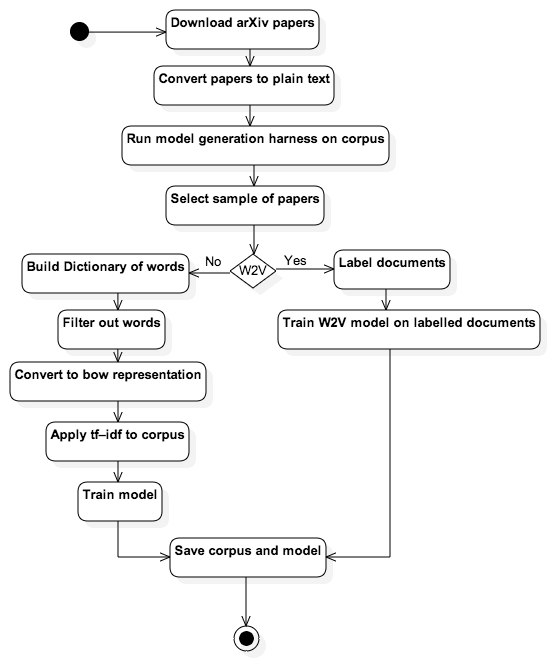
\includegraphics[width=10cm]{Figures/ArchictectureBuildingUML.png}
As shown in the UML activity diagrams the system has to go through a number of steps to build the models.
First the system has to download the papers from the arXiv amazon S3 bucket.
The papers are then converted from PDF to txt and sorted into directories based on their arXiv topic separations.
A harness for building the models is then run on the plain text corpus.
Depending on the algorithm used the system flow splits at this point.

If LDA or KNN is used then a dictionary of words must be built and then very common and very uncommon words are filtered out.
This is done as very common words that are present in a majority of the documents are very unlikely to have strong influence on the similarity of the content of documents.
Likewise very uncommon words are discarded as they are very likely to be noise in the dataset.
Examples of this would be misspelled words or typesetting errors from the original papers.

Once the dictionary is created a bag-of-words representation of the corpus is created.
A bag-of-words representation is one where a document is represented by a vector of tuples.
These tuples contain a word identification number and another number which represents the frequency of the word in that document.
A tf–idf (term frequency–inverse document frequency) transformation is then applied to the corpus.
The original bag-of-words representation created above, only models the term frequency of words in the document.
The inverse document frequency decreases in size the more often a particular word appears in the corpus as a whole.
A tf-idf transformation multiples the idf of a word with it's tf.
This results in the word being weighted by a value between 0 and 1 to show it's importance in the current document.
The LDA or the k-NN model is then trained using the tf-idf corpus.

When the algorithm being run is Word2Vec the documents do not need to be transformed into a bag-of-words representation as the neural network is trained on the document in their original context.
Word2Vec uses skip-gram architecture to train the neural network.
In the skip-gram architecture the neural network is fed word \(w_{i}\) and tries to fit to the outputs \(w_{i-1}\), \(w_{i-2}\), \(w_{i+1}\), \(w_{i+2}\).
The output words \(w_{i-1}\), \(w_{i-2}\), \(w_{i+1}\), \(w_{i+2}\) do not however have to be in the immediate vicinity of the word \(w_{i}\).
The output words can be in a user-defined window around the input word.

To train the Word2Vec model each of the documents are assigned a label which uniquely identifies that document.
The Word2Vec model is then trained on this labelled corpus.
This results in a model where each word and document in the corpus has a word vector representation.
This word vector representation can be used to query how similar words or documents are to each other.

\subsection{Queries}
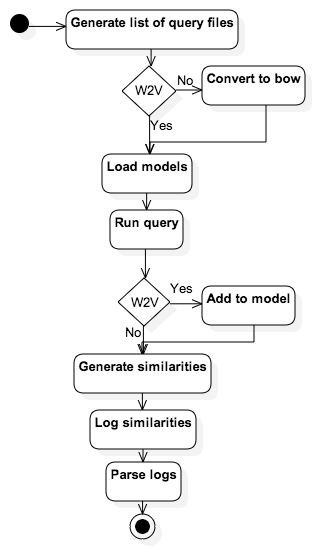
\includegraphics[width=15cm]{Figures/ArchictectureQueryUML.png}

\section{Conclusion}
